\documentclass[a4paper,10pt]{article}
%\documentclass[a4paper,10pt]{scrartcl}

\usepackage[utf8]{inputenc}
\usepackage{hyperref}

\title{Macro Buddy}
\author{Suciu Andrei}
\date{March 2025}


\pdfinfo{%
  /Title    (Software Design Project)
  /Author   (Suciu Andrei)
  /Creator  ()
  /Producer ()
  /Subject  ()
  /Keywords ()
}



\usepackage{graphicx}
\usepackage{listings}
\usepackage{xcolor}
\graphicspath{ {images/} }

\begin{document}
    \pagenumbering{gobble}
    \setlength{\parindent}{0pt}
    \begin{titlepage}
        \begin{center}
            \textbf{\large Department of Computer Science} \\[0.2cm]
            \textbf{\large Technical University of Cluj-Napoca} \\[0.5cm]
            
\includegraphics[width=1\textwidth]{utLogo.png} \\[1.0cm]

            \textbf{Software Design Project} \\
            \textit{Laboratory activity 2025} \\[4.0cm]

            Name: Suciu Andrei \\
            Group: 30431 \\
            Email: suciu.se.an@student.utcluj.ro\\

            \vfill

            Software Design \\[0.5cm]
            
\includegraphics[width=1\textwidth]{utLogo.png} \\[4.0cm]


        \end{center}
    \end{titlepage}
    \newpage

    \tableofcontents
    \newpage
    \pagenumbering{arabic}


\section{Deliverable 1}
    \subsection{Project Specification}
    Macro Buddy is a calorie tracking application designed to help users monitor their nutritional intake and achieve their dietary goals. The system allows users to track their daily food consumption by recording entries in a personal journal, organized by date and meal type. \\

    The application is built using Java Spring framework with a PostgreSQL database for data persistence, containerized using Docker. The current implementation includes a mock frontend developed with Java Swing, following the Model-View-Controller architectural pattern. \\

    Macro Buddy supports two types of users: regular users and administrators. Regular users can manage their personal food entries and customize their nutritional goals, while administrators have additional privileges to create and manage the food database accessible to all users.

    \newpage
    \subsection{Functional Requirements}
    \begin{enumerate}
        \item \textbf{User Authentication and Authorization}
        \begin{itemize}
            \item Users must be able to register with a unique username and email
            \item Users must be able to log in securely with their credentials
            \item The system must distinguish between regular users and administrators
            \item Access to certain functions must be restricted based on user role
        \end{itemize}

        \item \textbf{Food Database Management}
        \begin{itemize}
            \item Administrators must be able to create new food entries with nutritional information
            \item The system must store comprehensive nutritional data for each food item
            \item Users must be able to search and browse the food database
        \end{itemize}

        \item \textbf{Personal Journal Management}
        \begin{itemize}
            \item Users must be able to add and remove food entries to their personal journal
            \item Users must be able to specify date, meal type, and quantity for each entry
            \item Users must be able to view their entries filtered by date
        \end{itemize}

        \item \textbf{Nutritional Goal Setting}
        \begin{itemize}
            \item Users must be able to set personal nutritional goals for calories, protein, fat, and carbohydrates
            \item The system must provide default values for new users
            \item Users must be able to update their goals at any time
        \end{itemize}

        \item \textbf{Nutritional Analysis}
        \begin{itemize}
            \item The system must calculate and display daily totals of nutritional intake
            \item The system must compare daily totals against user goals
            \item The system must provide visual feedback on goal progress
        \end{itemize}
    \end{enumerate}

    \newpage
    \subsection{Use Case Model}

        \subsubsection{Use Cases Identification}
        \textbf{Use-Case:} User Registration\\
        \textbf{Level:} User goal\\
        \textbf{Primary Actor:} Unregistered User\\
        \textbf{Main success scenario:}
        \begin{enumerate}
            \item User provides username, email, and password
            \item System validates input data
            \item System creates new user account with regular user role
            \item System initializes default nutritional goals for the user
            \item System confirms successful registration
        \end{enumerate}
        \textbf{Extensions:}
        \begin{itemize}
            \item Invalid or duplicate username/email: System notifies user and requests different input
        \end{itemize}

        \textbf{Use-Case:} User Login\\
        \textbf{Level:} User goal\\
        \textbf{Primary Actor:} Registered User\\
        \textbf{Main success scenario:}
        \begin{enumerate}
            \item User provides username/email and password
            \item System authenticates credentials
            \item System grants access appropriate to user role
        \end{enumerate}
        \textbf{Extensions:}
        \begin{itemize}
            \item Invalid credentials: System notifies user and allows retry
        \end{itemize}

        \textbf{Use-Case:} Add Food Entry\\
        \textbf{Level:} User goal\\
        \textbf{Primary Actor:} Regular User\\
        \textbf{Main success scenario:}
        \begin{enumerate}
            \item User selects date and meal type
            \item User searches for food item from database
            \item User specifies quantity consumed
            \item System calculates nutritional values based on quantity
            \item System adds entry to user's journal
            \item System updates daily nutritional totals
        \end{enumerate}
        \textbf{Extensions:}
        \begin{itemize}
            \item Food item not found: User can request admin to add new food
        \end{itemize}

        \textbf{Use-Case:} Create New Food Item\\
        \textbf{Level:} User goal\\
        \textbf{Primary Actor:} Administrator\\
        \textbf{Main success scenario:}
        \begin{enumerate}
            \item Admin provides food name, producer, and serving information
            \item Admin inputs nutritional data (calories, protein, fat, carbs)
            \item System validates input data
            \item System adds new food item to database
            \item System confirms successful addition
        \end{enumerate}
        \textbf{Extensions:}
        \begin{itemize}
            \item Invalid or incomplete data: System highlights issues and requests corrections
        \end{itemize}

        \textbf{Use-Case:} Modify Nutritional Goals\\
        \textbf{Level:} User goal\\
        \textbf{Primary Actor:} Regular User\\
        \textbf{Main success scenario:}
        \begin{enumerate}
            \item User accesses personal settings
            \item User modifies calorie, protein, fat, and/or carb goals
            \item System validates input values
            \item System updates user's nutritional goals
            \item System recalculates progress based on new goals
        \end{enumerate}
        \textbf{Extensions:}
        \begin{itemize}
            \item Invalid values: System explains valid ranges and requests corrections
        \end{itemize}

        \newpage
        \subsubsection{UML Use Case Diagrams}
        \begin{figure}[h]
        \centering
        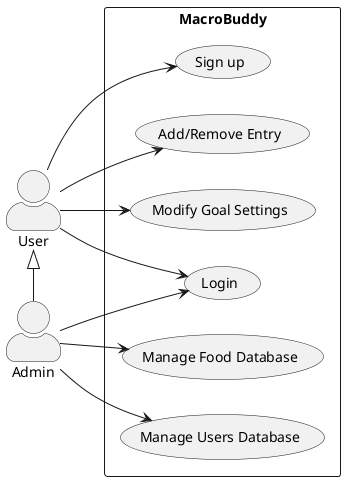
\includegraphics[width=0.7\textwidth]{uml.png}
        \caption{Macro Buddy Use Case Diagram}
        \end{figure}

    \newpage
    \subsection{Supplementary Specifiaction}

        \subsubsection{Non-Functional Requirements}
        \textbf{1. Security}

        The system must securely store user credentials and personal data. Passwords must be stored using cryptographic hashing algorithms. Access to user journals and personal data must be restricted to the respective users only. Administrator privileges must be strictly controlled. \\

        This requirement is suitable for implementation because:
        \begin{itemize}
            \item Nutritional tracking applications contain sensitive personal health information
            \item Spring Security framework provides robust and easy to use security features
        \end{itemize}

        \textbf{2. Usability}

        The user interface must be intuitive and require minimal training. Common tasks should be accomplishable in three clicks or less. The system must provide meaningful feedback for user actions and clear error messages when needed.  \\

        This requirement is suitable for implementation because:
        \begin{itemize}
            \item Daily use applications must have low friction to encourage consistent use
            \item Java Swing allows for fast development of clean and intuitive interfaces
        \end{itemize}

        \textbf{3. Performance}

        The system must be highly respond to user input under normal operating conditions. The application must operate efficiently with at least 100 concurrent users, with minimal overhead on the users. \\

        This requirement is suitable for implementation because:
        \begin{itemize}
            \item Response time directly usability
            \item Spring and PostgreSQL can be configured for high performance
            \item Database indexing and query optimization can be implemented
        \end{itemize}

        \textbf{4. Maintainability}

        The codebase must follow object-oriented design principles and established design patterns. The system architecture must support future extension of features without major refactoring. \\

        This requirement is suitable for implementation because:
        \begin{itemize}
            \item The current package structure already supports separation of concerns
            \item Service-oriented architecture allows for modular development
            \item Unit tests provide a foundation for sustainable maintenance
            \item Java Spring supports extensible application design
        \end{itemize}

        \subsubsection{Design Constraints}
        \textbf{Technology Stack}

        The system must be implemented using Java Spring framework for the backend services and PostgreSQL for data persistence. The current implementation requires Java Swing for the frontend interface. \\

        \textbf{Architectural Patterns}

        The backend must implement a layered architecture with clear separation between controllers, services, and repositories. This ensures maintainability and supports potential future migration to a web-based interface. \\

        \textbf{Development Process}

        Development must follow test-driven development practices, with unit tests required for all service classes. Mockito and JUnit Jupiter are the preferred testing frameworks. \\

        \textbf{Deployment Environment}

        The database must be containerized using Docker to ensure consistent development and deployment environments. The application must be configurable to connect to either a local or remote PostgreSQL instance. \\

    \subsection{Glossary}
    \begin{description}
    \item[Entry] A record of food consumption by a user, including date, meal type, food item, and quantity.
        \begin{itemize}
            \item Format: Object with date (timestamp), meal (string), quantity (float), food reference, and user reference
            \item Validation: Quantity must be positive
        \end{itemize}

    \item[Food Item] A nutritional data record for a specific food, including macronutrient information.
        \begin{itemize}
            \item Format: Object with name, producer, serving information, and nutritional values
            \item Validation: Name is required, nutritional values must be non-negative
        \end{itemize}

    \item[Macronutrients] The primary nutritional components tracked by the system: protein, fat, and carbohydrates.
        \begin{itemize}
            \item Format: Floating-point values measured in the food's respective serving units
            \item Validation: Values must be non-negative
        \end{itemize}

    \item[Nutritional Goals] User-defined targets for daily intake of calories and macronutrients.
        \begin{itemize}
            \item Format: Integer for calories, floating-point for protein, fat, and carbohydrates
            \item Validation: Values must be positive
        \end{itemize}

    \item[Meal Type] A categorization of food entries based on time of day or purpose.
    \begin{itemize}
        \item Format: String value (e.g., "Breakfast", "Lunch", "Dinner", "Snack")
        \item Validation: Must be one of the predefined meal types
    \end{itemize}

    \item[Regular User] A standard user who can manage their personal journal and settings.
        \begin{itemize}
            \item Format: User object with role set to "ROLE\_USER"
            \item Validation: Must have valid user credentials
        \end{itemize}

    \item[Administrator] A user with elevated privileges who can manage the food database.
        \begin{itemize}
            \item Format: User object with role set to "ROLE\_ADMIN"
            \item Validation: Must have valid user credentials
        \end{itemize}
    \end{description}

\newpage
\section{Deliverable 2}
    \subsection{Domain Model}
        \begin{figure}[h]
        \centering
        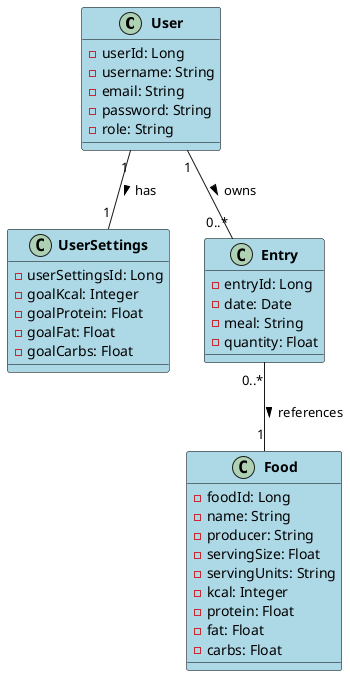
\includegraphics[width=0.6\textwidth]{domain_model.png}
        \caption{Macro Buddy Domain Model}
        \end{figure}

        The domain model illustrates the core entities of the system:

        \begin{itemize}
            \item \textbf{User}: Represents application users with authentication information and role designation (regular user or administrator).
            \item \textbf{UserSettings}: Contains the nutritional goals and other settings for a specific user.
            \item \textbf{Food}: Represents food items in the database with their nutritional information.
            \item \textbf{Entry}: Represents a food consumption record in a user's journal.
        \end{itemize}

        Key relationships:
        \begin{itemize}
            \item Each User has exactly one UserSettings profile.
            \item A User can have multiple Entry records (their food journal).
            \item Each Entry references exactly one Food item.
        \end{itemize}


    \subsection{Architectural Design}
        \subsubsection{Conceptual Architecture}
            The application implements client-server architecture with separation between the frontend and backend components. The backend follows a layered architecture pattern, while the frontend implements its own React-based architectural pattern. Together, they form a comprehensive web application with a React TypeScript frontend and a Java Spring RESTful API backend.

            \begin{figure}[h]
            \centering
            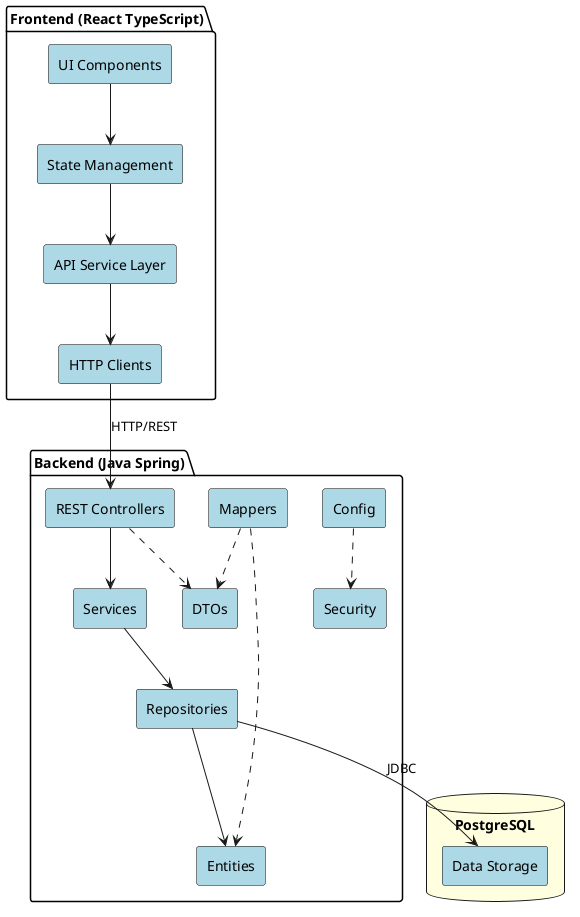
\includegraphics[width=0.6\textwidth]{conceptual_architecture}
            \caption{Conceptual Architecture}
            \end{figure}

            \newpage
            \textbf{Architectural Style Justification}:

            The client-server architecture with layered backend was chosen for the following reasons:

            \begin{enumerate}
                \item \textbf{Clear Separation of Concerns}: The architecture separates the frontend (React) from the backend (Spring) with a well-defined REST API interface between them. Within each part, there are further separations (UI components/services in frontend, controllers/services/repositories in backend).

                \item \textbf{Enhanced Security}: The architecture implements modern security practices with JWT for stateless authentication, CSRF protection for request verification, and secure password encryption.

                \item \textbf{Maintainability and Testability}: Each layer has clear responsibilities, making it easier to test components in isolation and update specific parts without affecting the entire system.
            \end{enumerate}

            The use of DTOs (Data Transfer Objects) and Mappers further enhances the architecture by:
            \begin{itemize}
                \item Providing a clear contract between frontend and backend
                \item Protecting internal domain objects from direct exposure
                \item Allowing for different representations of the same data for different use cases
            \end{itemize}
        \subsubsection{Package Design}
            The package structure reflects the layered architecture and organizes code by technical responsibility.

            \begin{figure}[h]
            \centering
            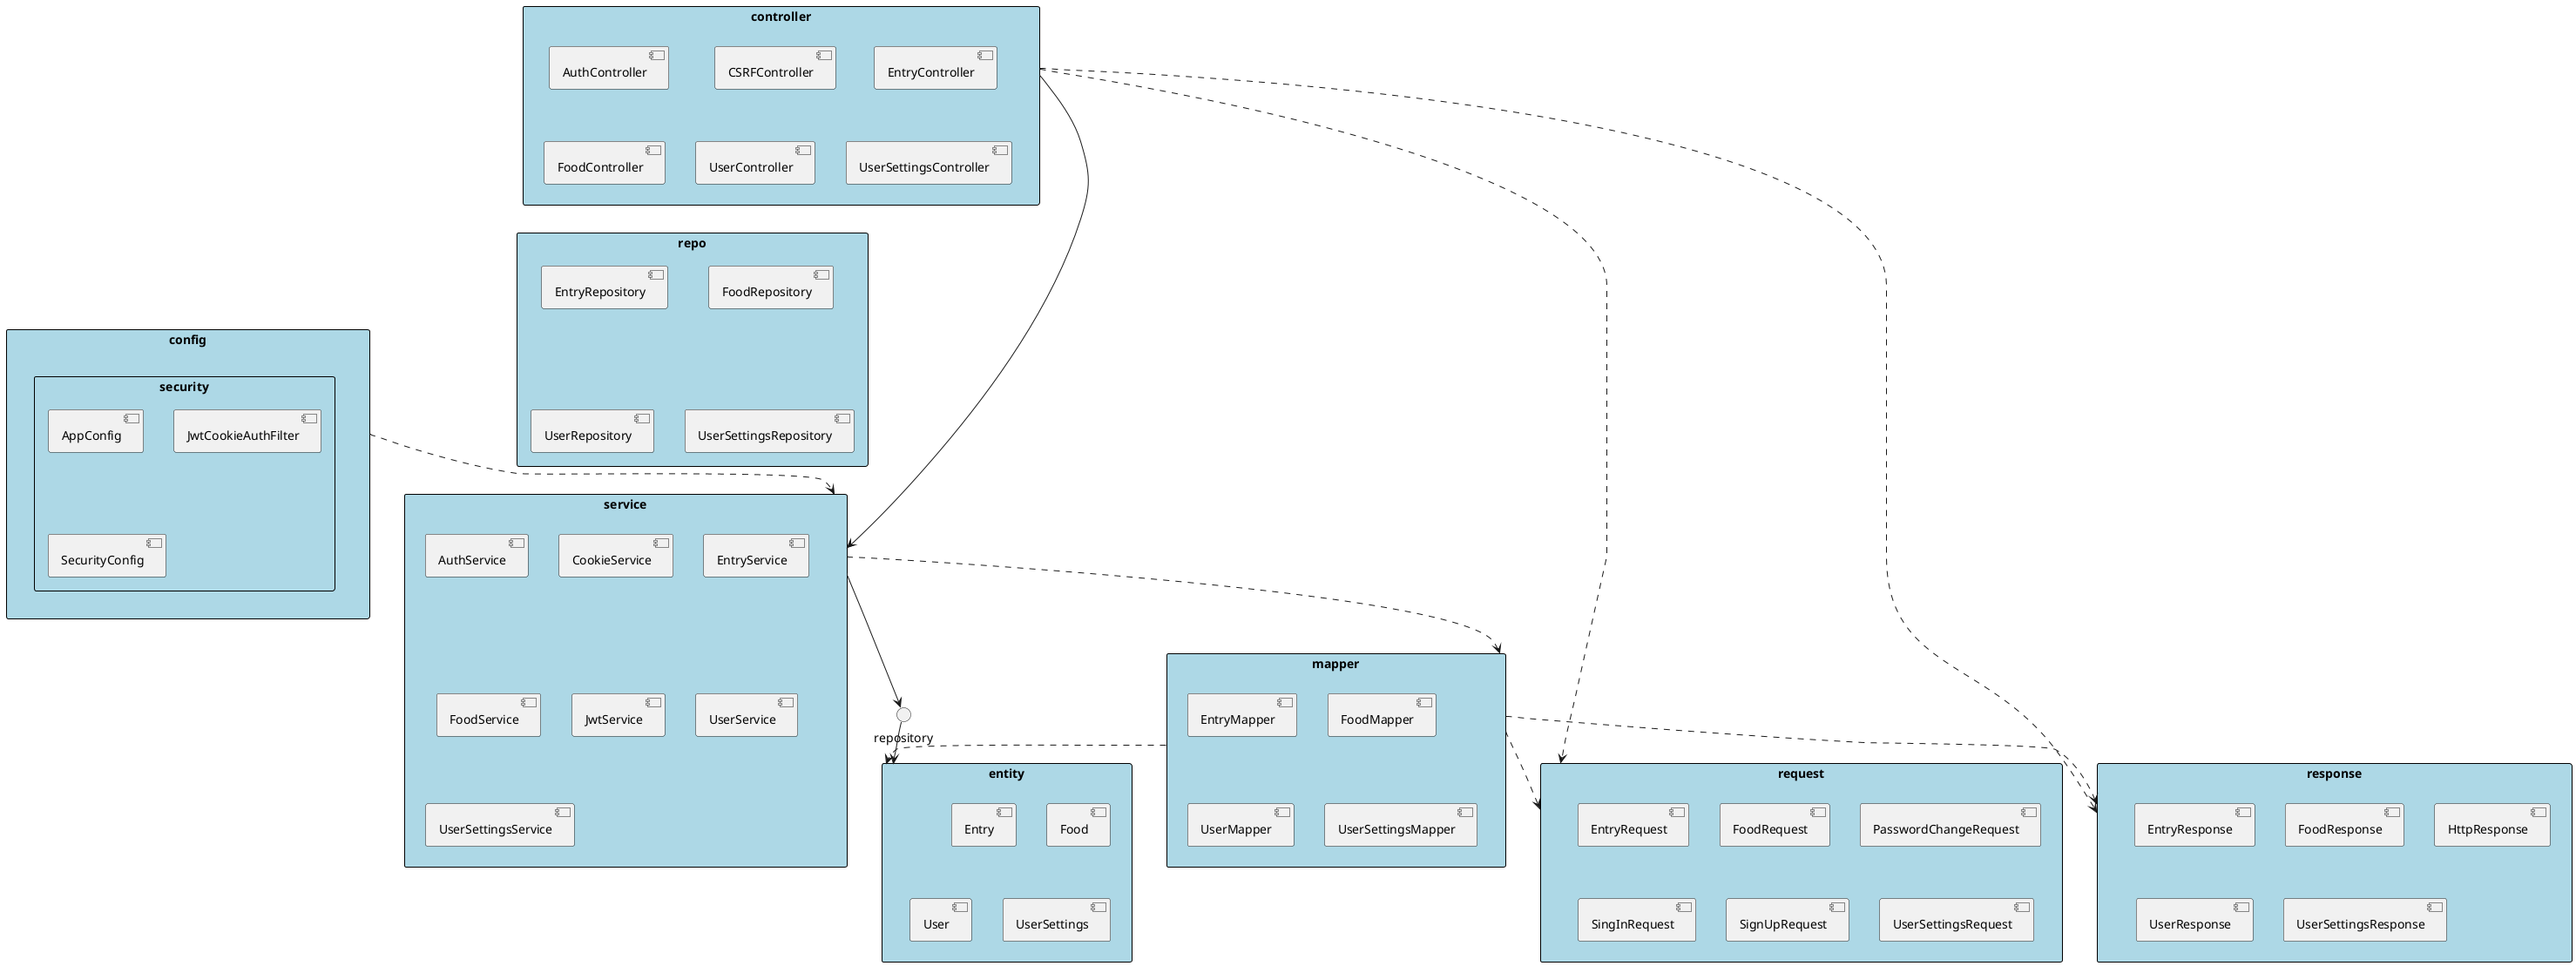
\includegraphics[width=0.8\textwidth]{package_diagram}
            \caption{Package Diagram}
            \end{figure}

            The package design follows a clear dependency direction, where higher-level packages (controller) depend on lower-level packages (service, repository), maintaining the layered architecture principles:

            \begin{itemize}
            \item \textbf{config}: Contains application configuration for security features (JWT, CSRF, password encryption)
            \item \textbf{controller}: REST API endpoints that handle HTTP requests and responses
            \item \textbf{service}: Business logic implementation
            \item \textbf{repo}: Data access layer for interacting with the database
            \item \textbf{entity}: JPA entity classes that map to database tables
            \item \textbf{mapper}: Converts between entities and DTOs
            \item \textbf{request/response}: DTOs for API input and output
            \end{itemize}

        \subsubsection{Component and Deployment Diagram}
            The component and deployment diagrams illustrate the runtime architecture and physical deployment structure of the system.

            \begin{figure}[h]
            \centering
            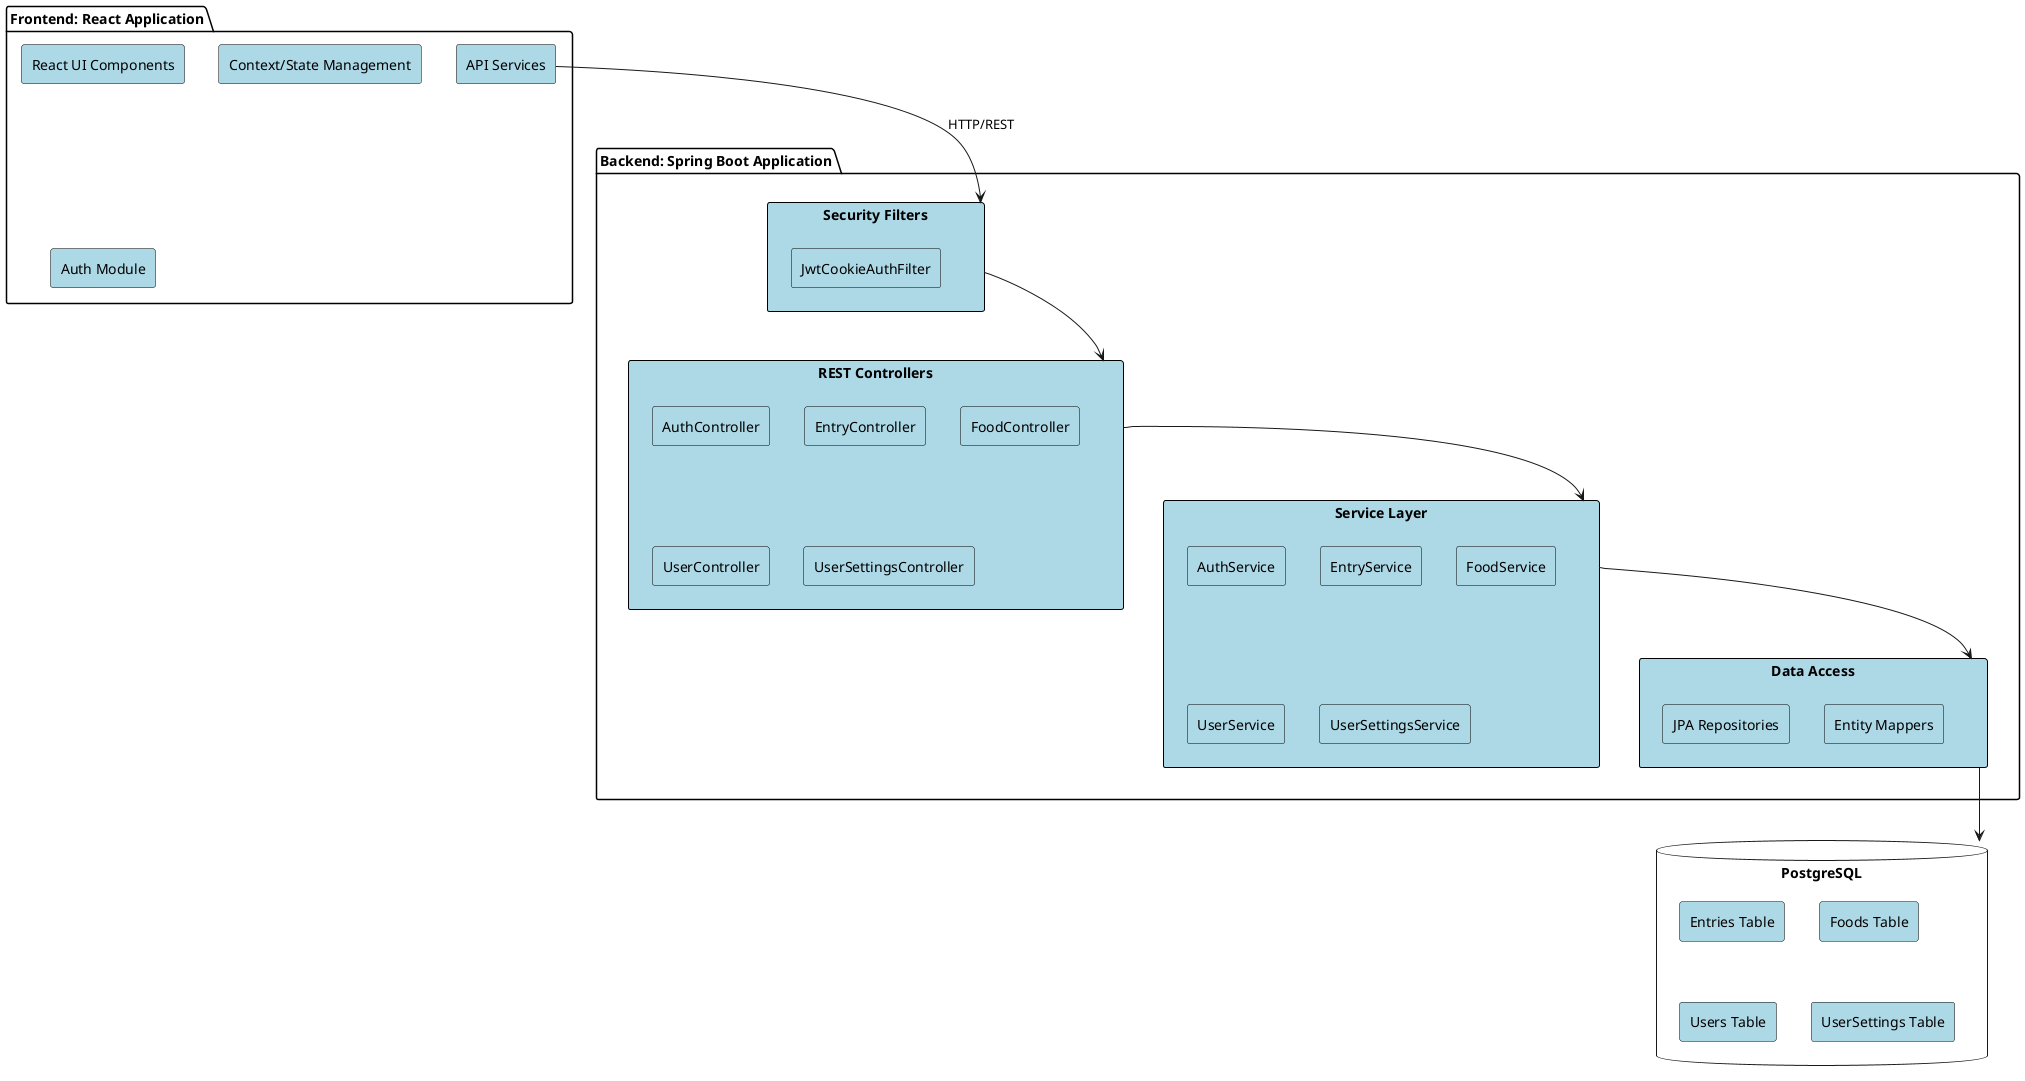
\includegraphics[width=0.8\textwidth]{component_diagram}
            \caption{Component Diagram}
            \end{figure}

            \begin{figure}[h]
            \centering
            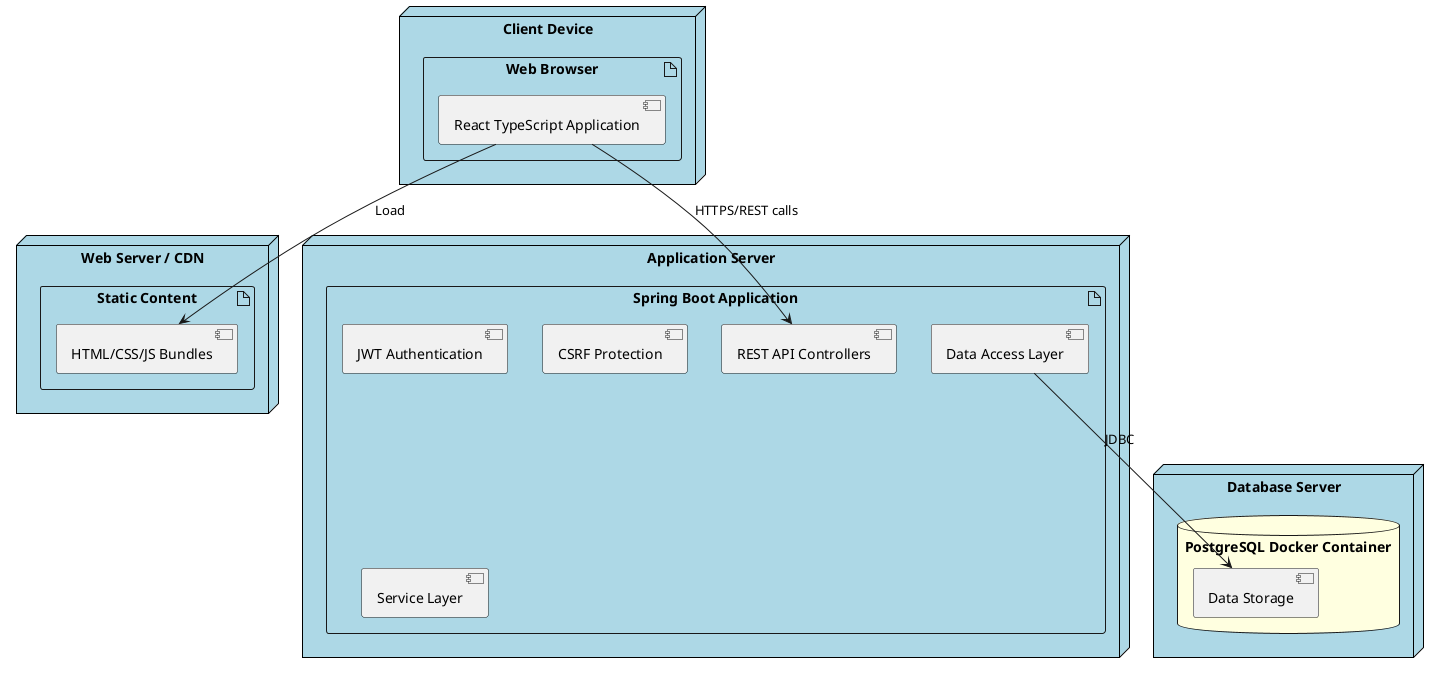
\includegraphics[width=0.8\textwidth]{deployment_diagram}
            \caption{Deployment Diagram}
            \end{figure}

            The component diagram shows the internal structure of the application with a focus on the logical components and their interactions, while the deployment diagram illustrates how these components are distributed across physical hardware or containerized environments.

            Key aspects of the deployment architecture:

            \begin{itemize}
                \item The frontend is a TypeScript React web application loaded in the client's browser.
                \item Static content (compiled React code) is served via a web server or CDN for optimal performance.
                \item The Spring Boot backend provides secure REST API endpoints with JWT authentication and CSRF protection.
                \item Business logic is implemented in the service layer, with clear separation from the data access layer.
                \item The PostgreSQL database runs in a Docker container for consistency across development and production environments.
                \item All client-server communication occurs via HTTP/S using RESTful conventions.
            \end{itemize}
\end{document}
